\chapter{IaaS}
Now we will consider the IaaS model in particular, this model allows full access to the resources
bought by the user, even though he's unable to control the cloud infrastructure, he controls
everything above (has very limited control on the network components).

Providers usually offer different servers with different operating systems that can be chosen by clients based on necessity. Now we will check all of the specific solutions on the market in specific.

\section{Amazon Web Services}
Amazon Web Services sells two different services which are Elastic Compute Cloud (EC2) and Simple
Storage Service (S3), one is a service that rents a virtual machine while the other is object
storage that is payed on a monthly basis.

AWS Cloud is available in more than 30 geographic regions and provides resizable compute capacity in the cloud, it's a pay per use service.

Thanks to the fact that Amazon in a gigantic company they can take avail of their strong presence on most markets to make sure that clients have the best possible experience in terms of reliability.

Also they offer a series of preconfigured templates for instances, so that spinning up a new machine in the cloud is as easy as looking for a specific virtual machine in a list. Amazon also offers the possibility to create virtual networks that are logically isolated from the rest of the AWS Cloud which can be optionally connected to the end user's network.

Amazon EC2 is hosted in multiple locations around the world and is composed by the following building blocks:
\begin{itemize}
    \item Regions
    \item Availability zones, multiple and isolated locations within each region
    \item Local zones, whic support the placeent of resources
    \item AWS Outposts, more native AWS services, infrastructure and operating models on-premises
    \item Wavelength zones, support developers in building applications that provide ultra-low latencies to 5G devices and end users.
\end{itemize}
The division into Regions is not only marketing related, each region is isolated and resources are tied to the region and only those resources can be seen/accessed from inside the Region. Each region has multiple isolated locations known as Availability Zones.

To launch an instance, the user selects a region and a virtual private cloud, and possibly a subnet from one of the availability zones. Availability Zones can make instances resilient to failures because if one instance fails the client can move traffic to another instance in another availability zone.

Amazon RDS enables the client to place resources, such as DB instances, and data in multiple locations.

An Outpost is a pool of AWS compute and storage deployed at a customer site.

Wavelength zones support developers in building applications that provide ultra-low latencies to 5G
devices and end users, it deploys standard AWS compute and storage services to the edge of
telecommunication carriers' 5G networks, a Wavelength Zone is deployed and tied to the region it's
being deployed in. Virtual Private Cloud can be extended to one or more Wavelength Zones.

AWS Greengrass is an open source edge runtime and cloud service for building, deploying, and managing device software. It allows to connect a variety of heterogeneous devices from minuscle sensors to large appliances.

AWS offers many more services as AWS GovCloud, which is an Amazon Region designed and developed to support security and compliance requirements of the US government.

\section{Microsoft Azure}
Azure offers more than 200 products and cloud services allowing many different interactions between the client and the provider.

Physical datacenters are arranged into regions and linked by one of the largest interconnected networks on the planet; the Azure cloud network can offer high availability, low latency and scalability.

the structure of the Azure cloud business is similar to the Amazon AWS one:
\begin{itemize}
    \item Azure datacenters are the physical buildings.
    \item Azure regions are sets of datacenters.
    \item Azure geography is a discrete market, typically containing at least one or more regions.
    \item Azure availability zones, unique physical locations within an Azure region and offer high availability to protect the client's applications nd data from datacenter failures.
\end{itemize}

\section{Open Nebula}
Open Nebula is an open source cloud and edge computing platform to build and manage enterprise clouds, it unifies public cloud simplicity and agility with private cloud performance, security and control.

Open Nebula provides unified management of IT infrastructure and supports both containers and applications. It integrates multiple virtualization technologies like VMware and KVM for fully virtualized clouds. It can easily deploy hybrid and edge environments connecting resources from different providers.

It consists of the cloud management cluster, with front-end nodes and the cloud infrastructure, made of one or several workload clusters. It's located at multiple geographical locations, edge clusters are deployed on premise and on public cloud or edge providers. The following is Open Nebula's architecture.
\begin{figure}
    \centering
    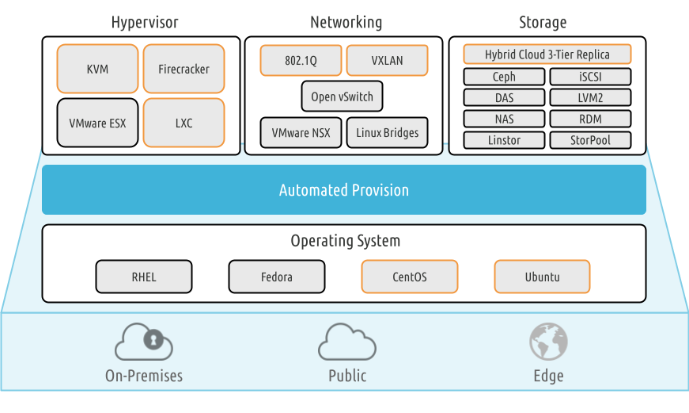
\includegraphics[scale=0.6]{img/Open_Nebula.png}
    \caption{Open Nebula's architecture}
\end{figure}

\section{OpenStack}
OpenStack is a cloud solution originally developed by NASA, it allows the creation and management of
public and private cloud operating systems that can control large pools of compute, storage and networking resources which are deployed and managed through an API or a dashboard.

OpenStack goes beyond standard IaaS functionally, it provides additional components, orchestration, fault management and service management amongst other services to ensure high availability of user applications. The following is the architecture of OpenStack.
\begin{figure}
    \centering
    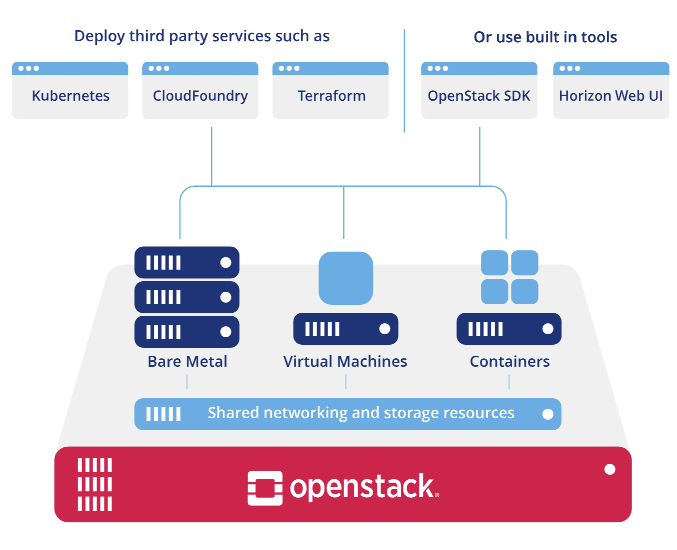
\includegraphics[scale=0.6]{img/OpenStack.png}
    \caption{OpenStack's architecture}
\end{figure}
OpenStack provides users with a trustworthy, configurable and open source cloud solution which is
easy to implement, provides scalability, extensibility and many advanced functionalities.

OpenStack's dashboard implements a GUI to retrieve, acess and automatize cloud resources, it permits the delivery of third party services like billing and monitoring. It provides an overview on the cloud dimension and status and permits to create users and projects, assigning users to projects and limit the use of resources. OpenStack provides a flexible architecture developed for horizontal scaling.

OpenStack is developed with horizontal scaling in mind and provides a flexible architecture.

When it comes to storage OpenStack supports both Object Storage and Block Storage:
\begin{itemize}
    \item Object storage provides storage with optimized costs and ability to scale out, it's nbot a traditional file system because it stores data in objects.
    \item Block storage permits to connect block devices to compute instances to achieve greater performance and integrates with enterprise storage platforms.
\end{itemize}
OpenStack's networking is scalable, based on APIs and is pluggable, which means that users can create their own network, control traffic and connect servers and devices.

The following is a diagram of the various OpenStack services.
\begin{figure}
    \centering
    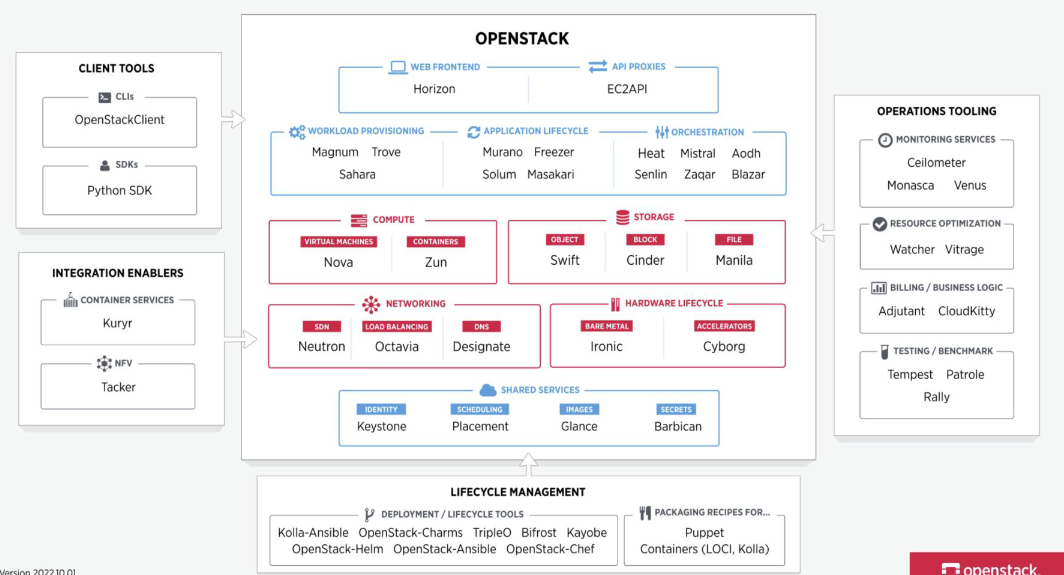
\includegraphics[scale=0.4]{img/OpenStack_Services.png}
    \caption{OpenStack services}
\end{figure}
OpenStack's dashboard, \textbf{Horizon}, is based on Django and can be accessed by clients and APIs
od any OpenStack services. Admin endpoints provide admin functionalities through the dashboard.

\textbf{Nova} is a fundamental service of OpenStack infrastructure, it manages the entire lifecycle of the VM instances in the virtualized environment. It handles horizontal scalability on standard hardware and can retrieve images needed for instance creation. Nova-network daemon is used for network management.

\textbf{Neutron} is a networking service that allows the creation and implementation in the virtual network of devices and interfaces managed by other OpenStack services. It interacts with the compute service to provide a network infrastructure and support network access to the instances.

The main operations are port plugging and unplugging, net and subnet creation and IP addressing.
Plug-in agenst differ on the basis of the provider and technologies ursed to implement the cloud
environment. Nova-network and Neutron are two different implementations of the
Networking-as-a-Service (NaaS) paradigm for OpenStack.

\textbf{Cinder} adds persistent storage to a VM, the data is maintained until the VM is canceled and provides an infrastructure to manage volumes and volume snapshots.

\textbf{Swift} is a multi-tenant object storage system, it's used to store data and images of VMs, data is maintained until the VM is cancelled and can be accessed everywhere. It provides abstractions to store methods, not storage itself.

\textbf{Keystone} has two main functions, it tracks users and corresponding privileges, it provides
a list of services available with API endpoint. Keystone generates authorization tokens for users.

\textbf{Glance} is the image manager, it accepts requests for disk images or server images, VMs, or metadata corresponding to images of end users or OpenStack compute components.

It supports provisioning from different types of repositories.

\textbf{Ceilometer} is the telemetry manager, it collects data from OpenStack services regarding different components of the infrastructure. It can send alarms when collected data violates predefined rules and contains:
\begin{itemize}
    \item Compute-agent
    \item Central-agent
    \item Notification-agent
    \item Collector
    \item Alarm evaluator
    \item Alarm notifier
    \item API server
\end{itemize}

\textbf{Heat} is the orchestration manager providing a template-based orchestration. Allows automation of the infrastructure deplyment. The template language allows to:
\begin{itemize}
    \item Specify virtual machine configurations (compute, storage and network)
    \item Specify post-deployment activities
    \item Create many types of OpenStack resources
\end{itemize}
Heat allows developers to directly integrate the orchestration module via a custom plug-in.

OpenStack contains four different networks:
OpenStack contains four different networks:
\begin{itemize}
    \item Management network - dedicated to internal communications between the processes, the IPs
        in this network are reachable only inside the datacenter.
    \item Data network - used for VM data communication within the cloud deployment.
    \item External network - used to provide VMs with internet access in some deployment scenarios,
        the IPs should be accessible by anyone on the internet.
    \item API network - which exposes OpenStack APIs.
\end{itemize}
The way they interact with the OpenStack system is summarized in Figure \ref{fig:openstack-network}
\begin{figure}
    \centering
    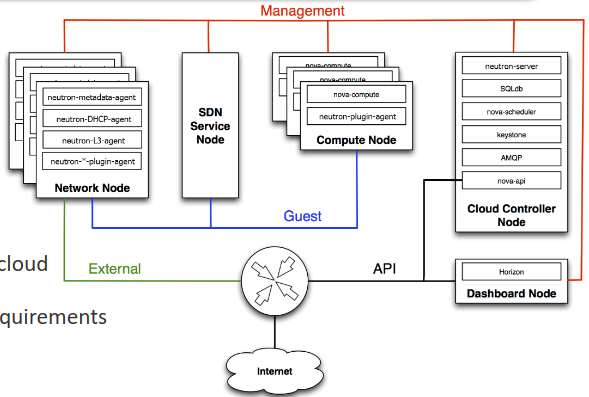
\includegraphics[scale=0.5]{img/OpenStack_network.png}
    \caption{The OpenStack networks}
    \label{fig:openstack-network}
\end{figure}

All services authenticate using the identity service and interact through public APIs (apart from
the privileged admin commands), the communication between different processes is handled through an
advanced message queuing protocol, which is a glorified message broker and the service status is
stored in a database.

An example of usecase for OpenStack is the one of BigData.
